\begin{figure}[!h]
\centering
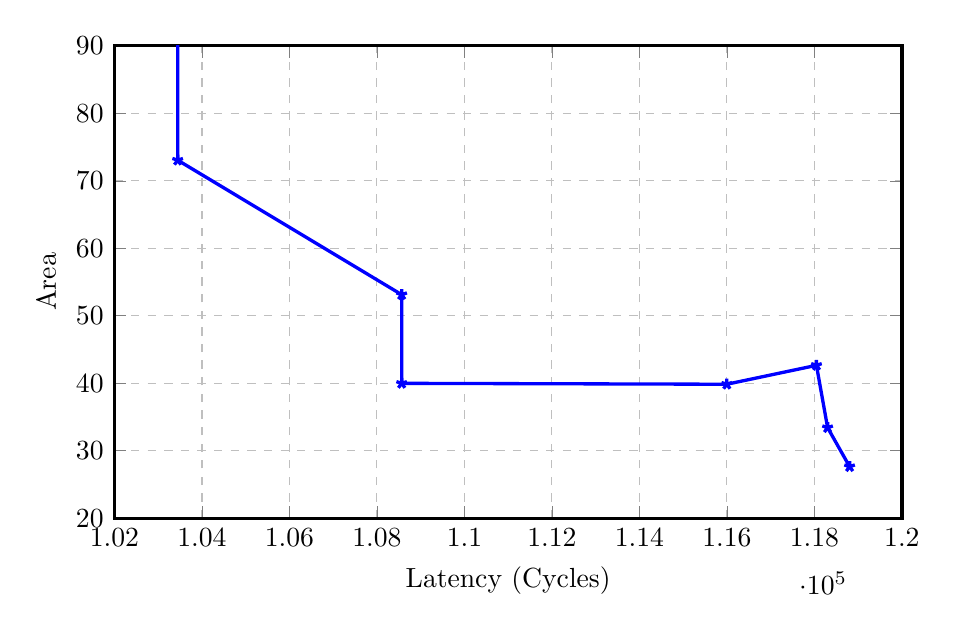
\begin{tikzpicture}
\begin{axis}[
scale only axis,
height=6cm,
width=10cm,
    xlabel={Latency (Cycles)},
    ylabel={Area},
    xmin=102000, xmax=120000,
    ymin=20, ymax=90,
    xtick={102000,104000,106000,108000,110000,112000,114000,116000,118000,120000},
    ytick={20,30,40,50,60,70,80,90},
    legend pos=north east,
    ymajorgrids=true,
    xmajorgrids=true,
    grid style=dashed,
    very thick
]
\addplot[
    color=blue,
    mark=star,
   % smooth
    ]
    coordinates {
    (103445,90.154)(103445,73.054)(108565,53.129)(108565,39.9875)(115998,39.854)(118047,42.654)(118302,33.425)(118805,27.646)
    };
\end{axis}
\end{tikzpicture}
\caption{Area Vs. Latency Curve for 1024-Point FFT Implementation}
\label{plot_1024fft}
\end{figure}